\begin{figure}[thb]
  \centering
  \begin{minipage}{1.0\hsize}
    \begin{center}
      \includegraphics[width=15cm]{chapter2/pomdp.eps}
      \caption{部分観測マルコフ決定過程(POMDP)の流れ}
      \label{fig:pomdp}
      \hspace{1.6cm}
    \end{center}
  \end{minipage}
  \begin{minipage}{1.0\hsize}
    \begin{center}
      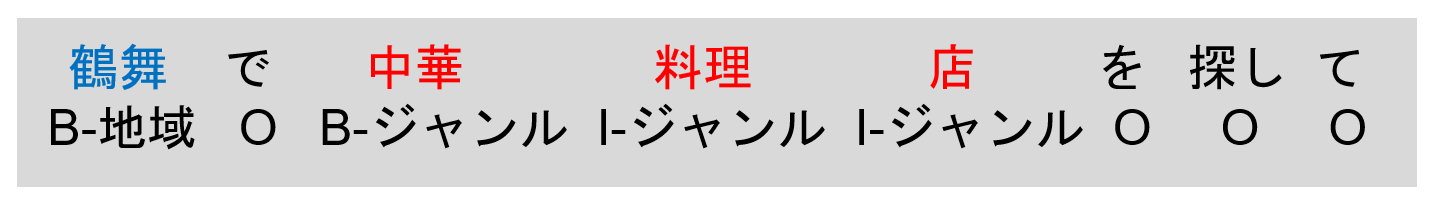
\includegraphics[width=15cm]{chapter2/crf.eps}
      \caption{IOBタグを用いたスロット抽出}
      \label{fig:crf}
    \end{center}
  \end{minipage}
\end{figure}

機械学習による対話システムにおいて,対話状態 $s_t$ はユーザ発話の解釈に不確実性が存在するため直接観測することはできないとしている.それゆえ図\ref{fig:pomdp}のように,言語理解部の出力をノイズを含むユーザ入力の観測 $o_t$ と見なして確率 $p(o_t|s_t)$ と表し,対話状態は全ての対話状態にわたる確率分布である信念 $b_t$ で表す.そして,言語理解部には条件付き確率場(Conditional
Random Field ; CRF)\cite{crf}と呼ばれる統計的機械学習を用いて,対話管理部には部分観測マルコフ決定過程(Partially Observable Markov Decision Process ; POMDP)\cite{pomdp}と呼ばれる強化学習を用いる.
\par
CRF は無向グラフにより表現される確率的グラフィカルモデルの1つであり,識別モデルである.無向グラフは方向性のないエッジ(辺)とノード(頂点)からなるグラフのことで,確率的グラフィカルモデルはグラフが確率変数間の条件付き依存関係を示すような確率モデルを指す.このモデルでは,ノードを確率変数,エッジを依存関係を表す.また,識別モデルとはあるデータがどのクラスに属するかを確率で表すモデルを指す.
\par
CRFは系列ラベリングというタスクに取り組むための手法である.系列ラベリングというのは,単語列のようなデータ列を入力として,個々のデータにラベルを付加するタスクのことである.言語理解におけるスロット抽出では,IOBタグと呼ばれるラベルが用いられる.IOBタグは,図\ref{fig:crf}のように B がスロット値の開始地点を示し,I がスロット値の継続を示し,O がスロット値でないことを示す.そして,スロット値抽出後には事前定義した辞書によって単語の差異を取り除く(例:「中華料理店」$\rightarrow$ 「中華料理」).
\par
ここから POMDP による対話管理の説明を行う.POMDP が使われ始めた経緯には,音声認識結果や言語理解結果に誤りが含まれ,対話状態に確実性がなかったことが挙げられる.よって,図\ref{fig:pomdp}に示した通り,統計的機械学習モデルでは,対話状態$s$ではなく全ての対話状態にわたる確率分布を持つ信念$b$で対話状態を表す.そして,言語理解部の出力$P(o'|s')$ と信念$b$を用いた状態更新関数によって最新の信念$b'$に更新する.その後,政策関数$\pi (b)$を用いてシステムの対話行為$a$を決める.POMDP では信念と対話行為から報酬を計算し,政策関数を強化学習により最適化していく.POMDP の問題は,複雑なタスクや複数のタスクを取り扱うと対話状態のパターンが増加するため,信念の計算量が膨大になること,ルールベースほどではないが言語理解部以前の誤りから悪影響を受けることなどが挙げられる.